\begin{IEEEbiography}[{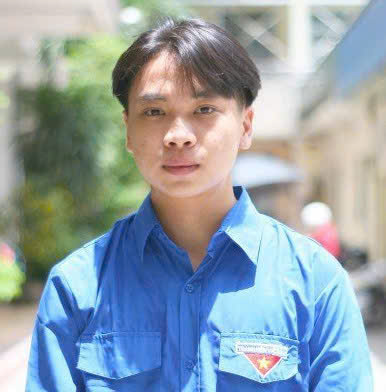
\includegraphics[width=1in,height=1.25in,clip,keepaspectratio]{images/author/author_thong_luc.jpg}}]{Thong Luc}
Thong Luc is a final-year undergraduate student in the B.Sc. program in Computer Science with the Faculty of Information Technology, University of Science, Vietnam National University Ho Chi Minh City, Vietnam. His research interests include computer vision, deep learning, medical image analysis, image segmentation, and interactive prompt-guided segmentation. His current work focuses on prompt-guided segmentation for bone radiographic images using deep learning.
\end{IEEEbiography}

\begin{biographynophoto}{Nguyen Huu Binh}
Nguyen Huu Binh is currently an undergraduate student in Computer Science with the Faculty of Information Technology, University of Science, Vietnam National University Ho Chi Minh City, Vietnam. His research interests include computer vision, deep learning, and image segmentation. His current research focuses on deep learning methods for medical image segmentation using visual prompts.
\end{biographynophoto}

\begin{IEEEbiography}[{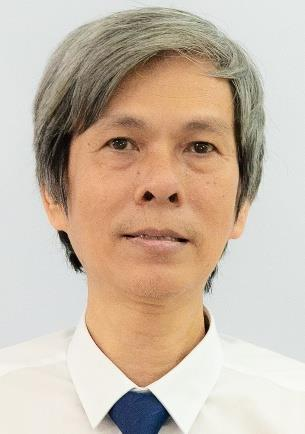
\includegraphics[width=1in,height=1.25in,clip,keepaspectratio]{images/author/author_ly_quoc_ngoc.jpg}}]{Ly Quoc Ngoc}
Ly Quoc Ngoc (Associate Professor, Ph.D.) is Head of the Department of Computer Vision and Cognitive Cybernetics, Faculty of Information Technology, University of Science, Vietnam National University Ho Chi Minh City, Vietnam. He received the B.Sc. degree in Mechanics and Mathematics, the M.Sc. degree in Computer Science, and the D.Sc. degree in Computer Science, all from the University of Science, Ho Chi Minh City, in 1987, 1996, and 2009, respectively. His research interests include artificial intelligence, machine learning, computer vision, digital image and video processing, computer graphics, multivariate statistical analysis, and medical image analysis. He has authored or co-authored nearly 70 papers in conference proceedings and academic journals, and has served as principal investigator of several research projects in intelligent vision systems.
\end{IEEEbiography}

